\begin{figure}[ht]
\begin{center}
 \begin{ccTexOnly}
   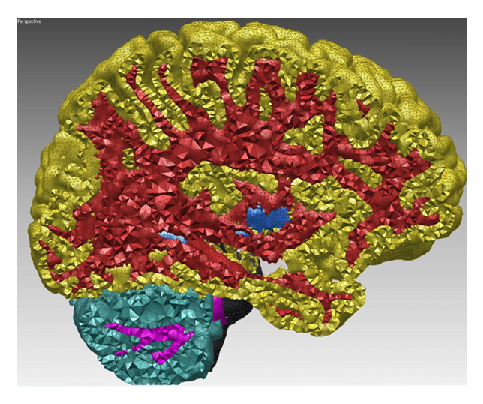
\includegraphics[height=9cm]{Mesh_3/pictures/multilabel_mesher}
 \end{ccTexOnly}
 \begin{ccHtmlOnly}
   <img border="0" src="./pictures/multilabel_mesher.jpg"><br/>
 \end{ccHtmlOnly}
 \caption{Cut-view of a multi-domain 3D mesh generated from a segmented image.}
  \label{figure:multilabel_mesher}
\end{center}
\end{figure}

\section{Introduction}
\label{Mesh_3_section_intro}

This package is devoted to the generation of  isotropic tetrahedron
meshes discretizing 3D domains. The main entry points of this component are
two global  functions that respectively generate
and refine such meshes.
%The main component of this package is a function which 
%generates 3D  simplicial meshes.
The domain to be discretized may be
formed either by a single connected component
or by several
connected components. We refer to the domain as a multi-domain
when the different components need to be
 identified  as different subdomains.
The mesh generator generates at once a simplicial 
3D mesh which includes one submesh for each subdomain
and surface meshes which approximate the boundaries 
 of the domain and subdomains.


\subsubsection{Input domain}

More specifically, the domain to be discretized is assumed
 to be representable as a pure
3D complex. A 3D complex is a set of faces with dimension
0 (vertices), 1 (edges), 2 (facets) and 3 (cells) such that
all faces are pairwise interior disjoint, 
and the boundary of each face of the complex is the union of faces
of the complex.
The 3D complex is pure, meaning that each face is included in a face of dimension 3,
so that the complex is entirely described as a set of 3D cells.
The set of faces with dimension lower or equal than 2 form a 2D
subcomplex. In the rest of the documentation, we will refer to the
input 3D complex as to the input domain.


Note that the input complex faces are not required to be linear. 
Facets, for instance, are typically smooth surface patches, 
or portion of surface meshes with boundaries.
The mesh generator provides at the same time
a 3D mesh discretizing each of the complex cells
and a surface mesh approximating the 2D complex 
that describes cell boundaries.
In its current state the mesh generator does not handle
sharp creases in the domain description. This does not mean  that 
the domain to be meshed  and its subdomains
are required to have smooth boundary surfaces.  The domain 
and  subdomains  boundaries  may be provided
 as smooth patches joined  along sharp edges.
However, currently, the mesh generator
 does  not take into account  the  edge description and hence
those edges are not  accurately  represented by a sequence of  mesh edges.


The mesh generator is able to handle
multiple junctions where three or more subdomains meet.
Consequently  the generated surface mesh may be non-manifold
as a whole, even if each  submesh approximating the boundary of a subdomain
is manifold.




The domain is input to the mesh generation function,
as a class 
devised to  answer queries about the domain as well as its subdomains.
Mainly, this class provides predicates which state
if  a given query point belongs 
to the domain or not, 
and in the affirmative, to which of the subdomains it belongs.
The current implementation provides  classes to represent
domains defined by implicit functions, polyhedral domains
and domains defined through 3D labeled images.

% The resulting mesh is output as a subcomplex of a 3D triangulation,
% in the form of a class providing various output iterators
% on mesh elements.

\subsubsection{Output mesh}

The resulting mesh is output as a subcomplex of a 3D triangulation,
in a class  providing various iterators
on mesh elements. The 3D triangulation provides an approximation of the
domain, subdomains and their boundaries, according to the restricted
Delaunay triangulation paradigm. This means that the domain
(resp. each subdomain) is approximated by the union of  the tetrahedral cells
 whose circumcenters are located inside the domain
(resp. inside the subdomain). 
Each surface patch of the domain or subdomains boundary is approximated
by the union of   the Delaunay facets whose dual Voronoi edges intersect the surface patch.
Such facets are called in the following {\em surface facets} or {\em boundary facets}. 

\subsubsection{Delaunay refinement}
\label{introsec:param}

The mesh generation algorithm is a Delaunay refinement process
followed by an optimization  phase.
%  which is currently implemented
% using the  sliver exudation approach~\cite{cgal:cdeft-slive-00}.
The   Delaunay refinement process is driven by criteria
concerning either the mesh cells 
or the surface facets.
%i.e., the facets of the mesh whose role is to approximate surface patches.
The refinement process terminates when there are
no more mesh cells or  surface facets violating the user-specified criteria.
The Delaunay refinement eliminates all kind of 
 badly shaped tetrahedra except slivers.
At the end of the refinement process,
some sliver shaped tetrahedra may occur in the mesh.
The optimization phase aims at eliminating slivers.

The criteria can  be tuned  to achieve the user needs with respect to
the size of mesh elements, the accuracy of boundary approximation
and topological conditions.
The default criteria  for surface facets are governed by the three following
parameters:
% \subsection{Parameters}
% \label{introsec:param}
%
% Some parameters are given to the refinement process to customize
% the generated mesh. Actually, each parameter correspond to a criteria
% that must be fullfilled by either each surface facet (if it is a
% \emph{surface facet parameter}) or each tetrahedron (if it is a
% \emph{cell parameter}). The mesh generation process ends when there is
% no more \emph{bad facet} or \emph{bad cell} given these criteria.
%
% In this package, we provide the following criteria. Note that each criteria may be
% deactivated by setting it to $0$.
%
%\subsubsection{Surface facet Parameters}
\begin{itemize}
\item \emph{the angular bound:} This parameter controls the shape of  
  surface facets. Actually, it is a lower bound for the angle (in degree) of
   surface mesh facets. The termination  of the meshing process is
guaranteed  if the angular bound is at most 30
  degrees. 
\item \emph{the radius bound:}  This parameter controls the size (edge
  length) of surface facets. Actually, each surface facet has 
a surface Delaunay ball which is a ball circumscribing the surface facet and
  centered on the surface patch.
 The radius bound is an upper 
  bound on the radii of surface Delaunay balls.
 \item \emph{the distance bound:}  This parameter controls the approximation error of the surface.
 Actually, it is an upper bound for the distance between the circumcenter
 of a surface facet and the center of a surface Delaunay ball of this facet.
\end{itemize}

%\subsubsection{Cell Parameters}
The default criteria for mesh cells are governed by two parameters:
\begin{itemize}
\item \emph{the radius-edge bound:}   This parameter controls the
  shape of mesh cells (but can't filter slivers, as we discussed earlier).
 Actually, it is an upper bound for the ratio
 between the circumradius of a 
   mesh tetrahedron and its shortest edge.
\item \emph{the radius bound:}  This parameter controls the size (edge length) of 
  mesh cells. Actually, it is an upper bound on the circumradii of the
 mesh tetrahedra.
\end{itemize}

Figure~\ref{figure:parameters} shows how the mesh generation process
behaves with respect to these parameters.

\begin{figure}[ht]
\begin{center}
 \begin{ccTexOnly}
   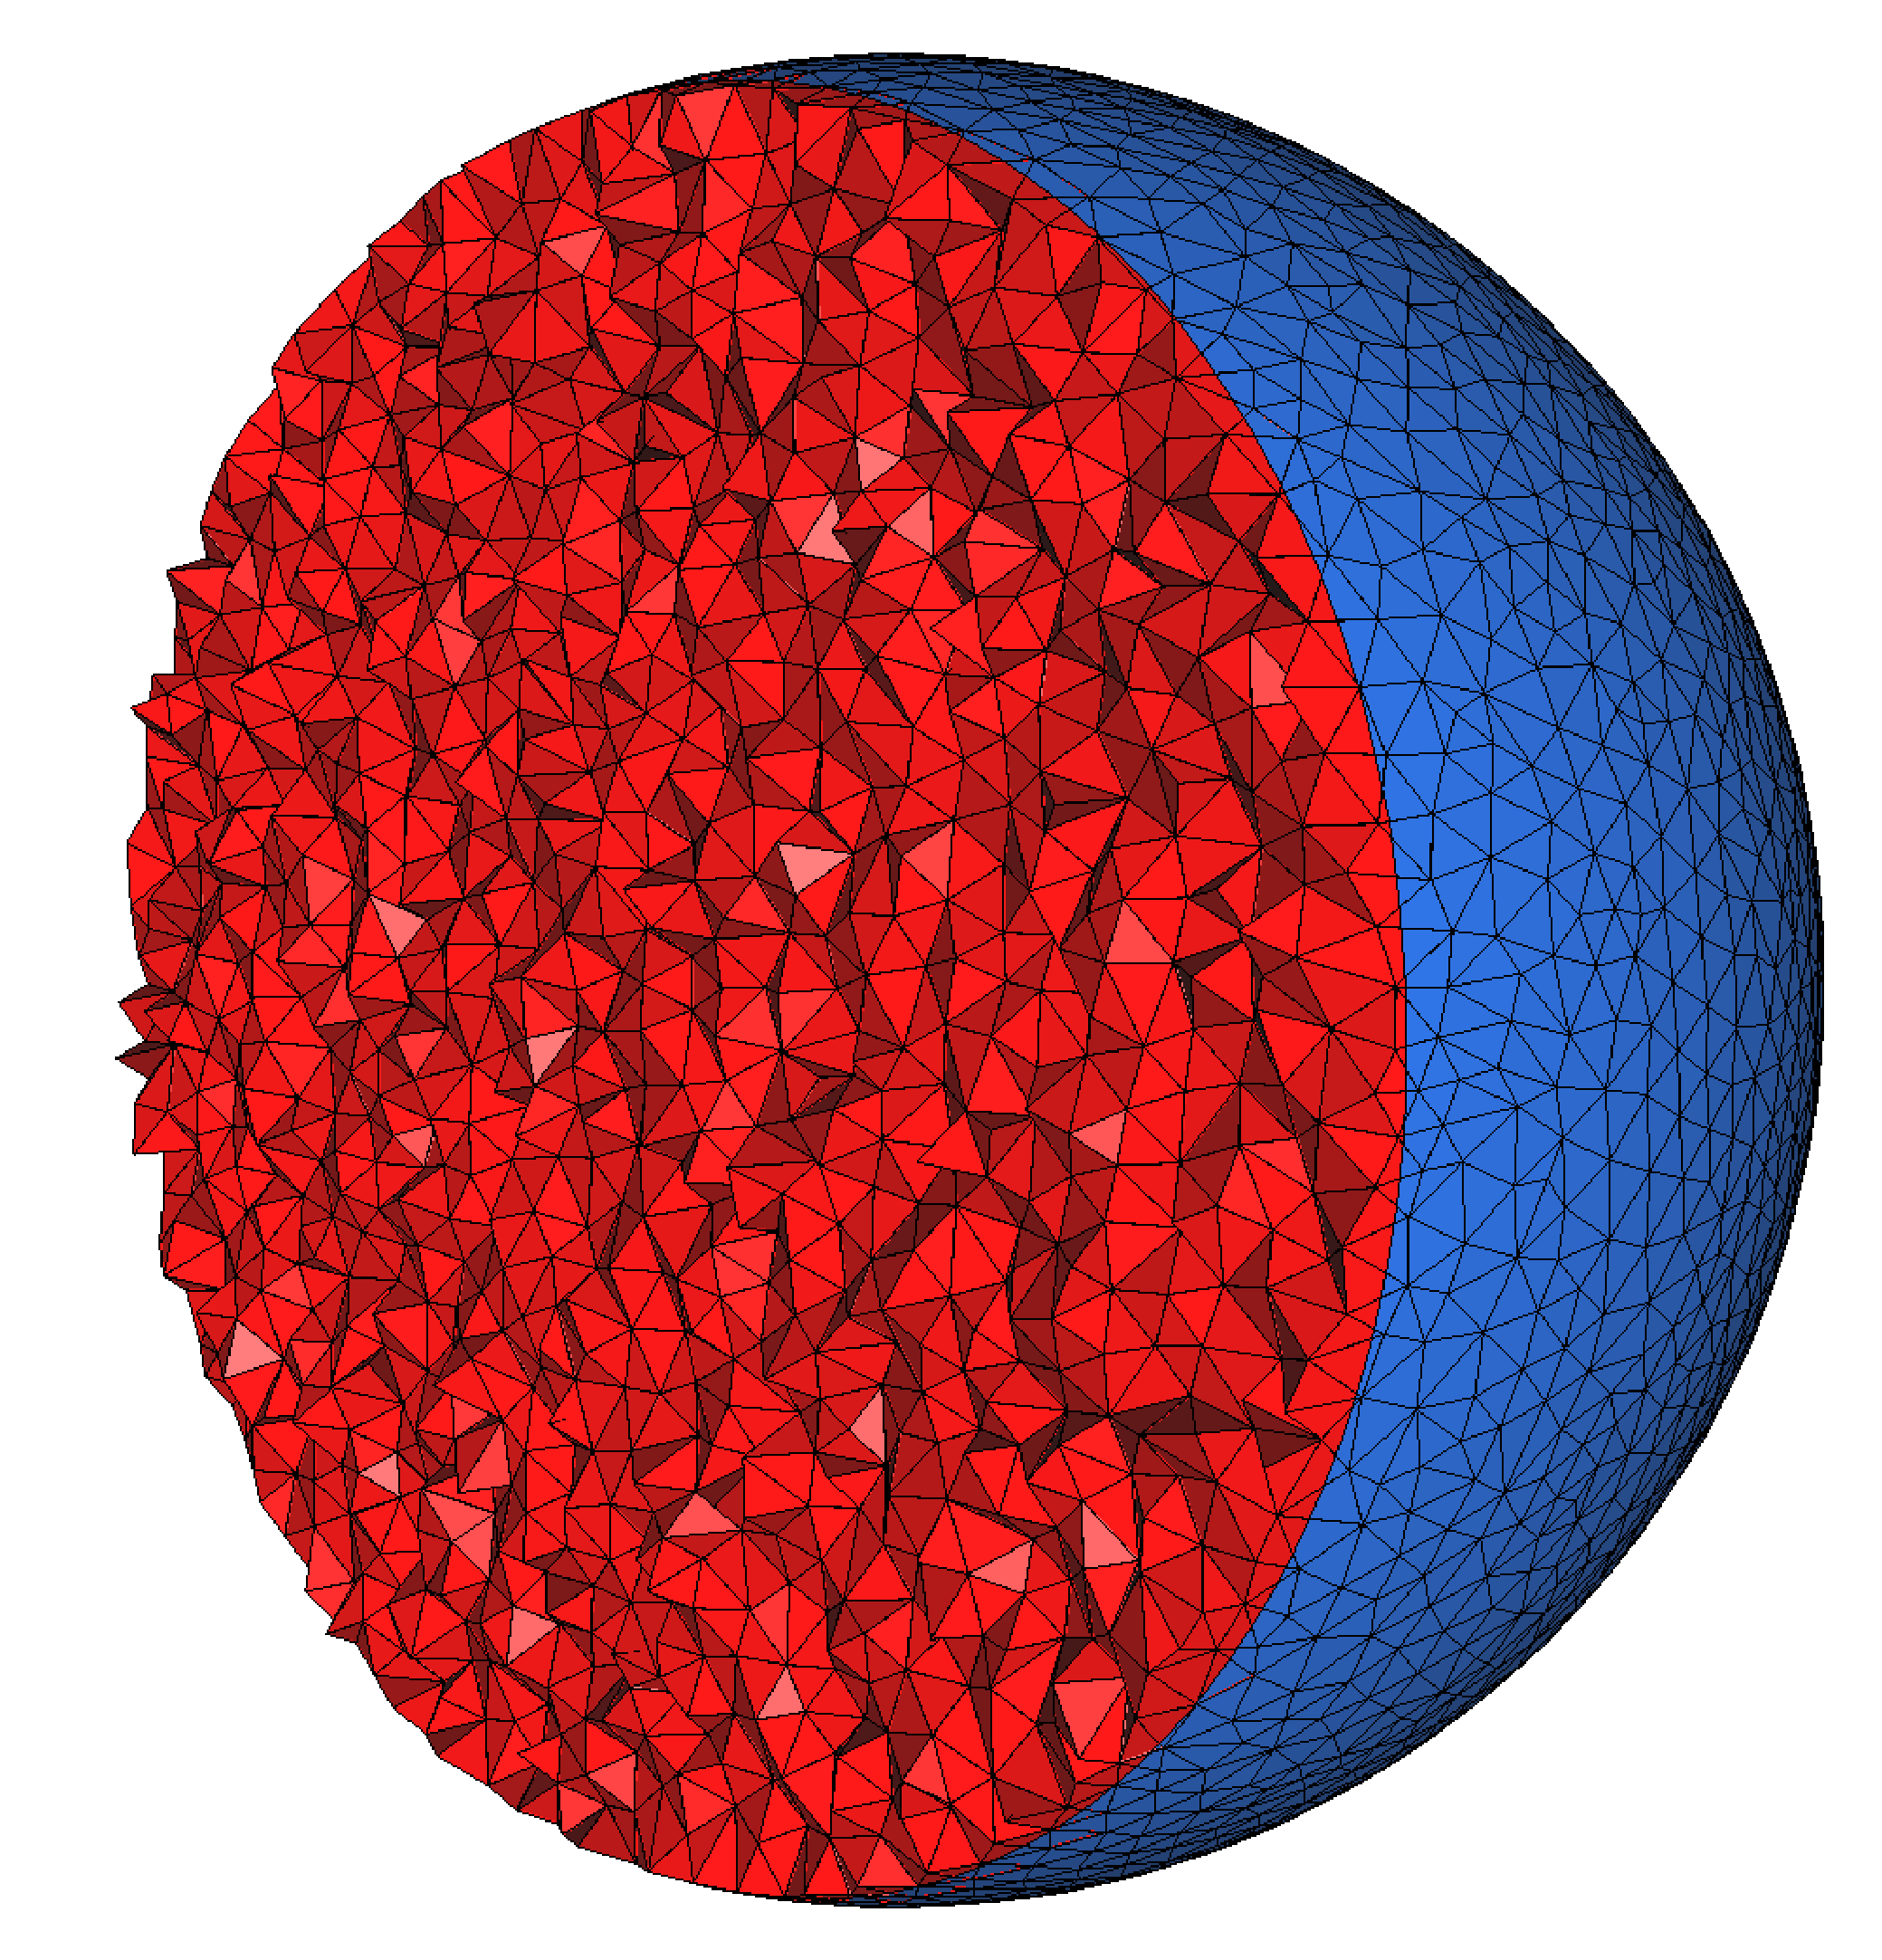
\includegraphics[height=5cm]{Mesh_3/pictures/implicit_domain}

   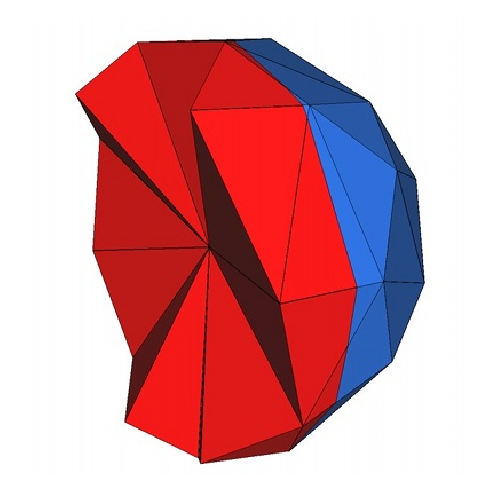
\includegraphics[height=5cm]{Mesh_3/pictures/implicit_domain_3}
   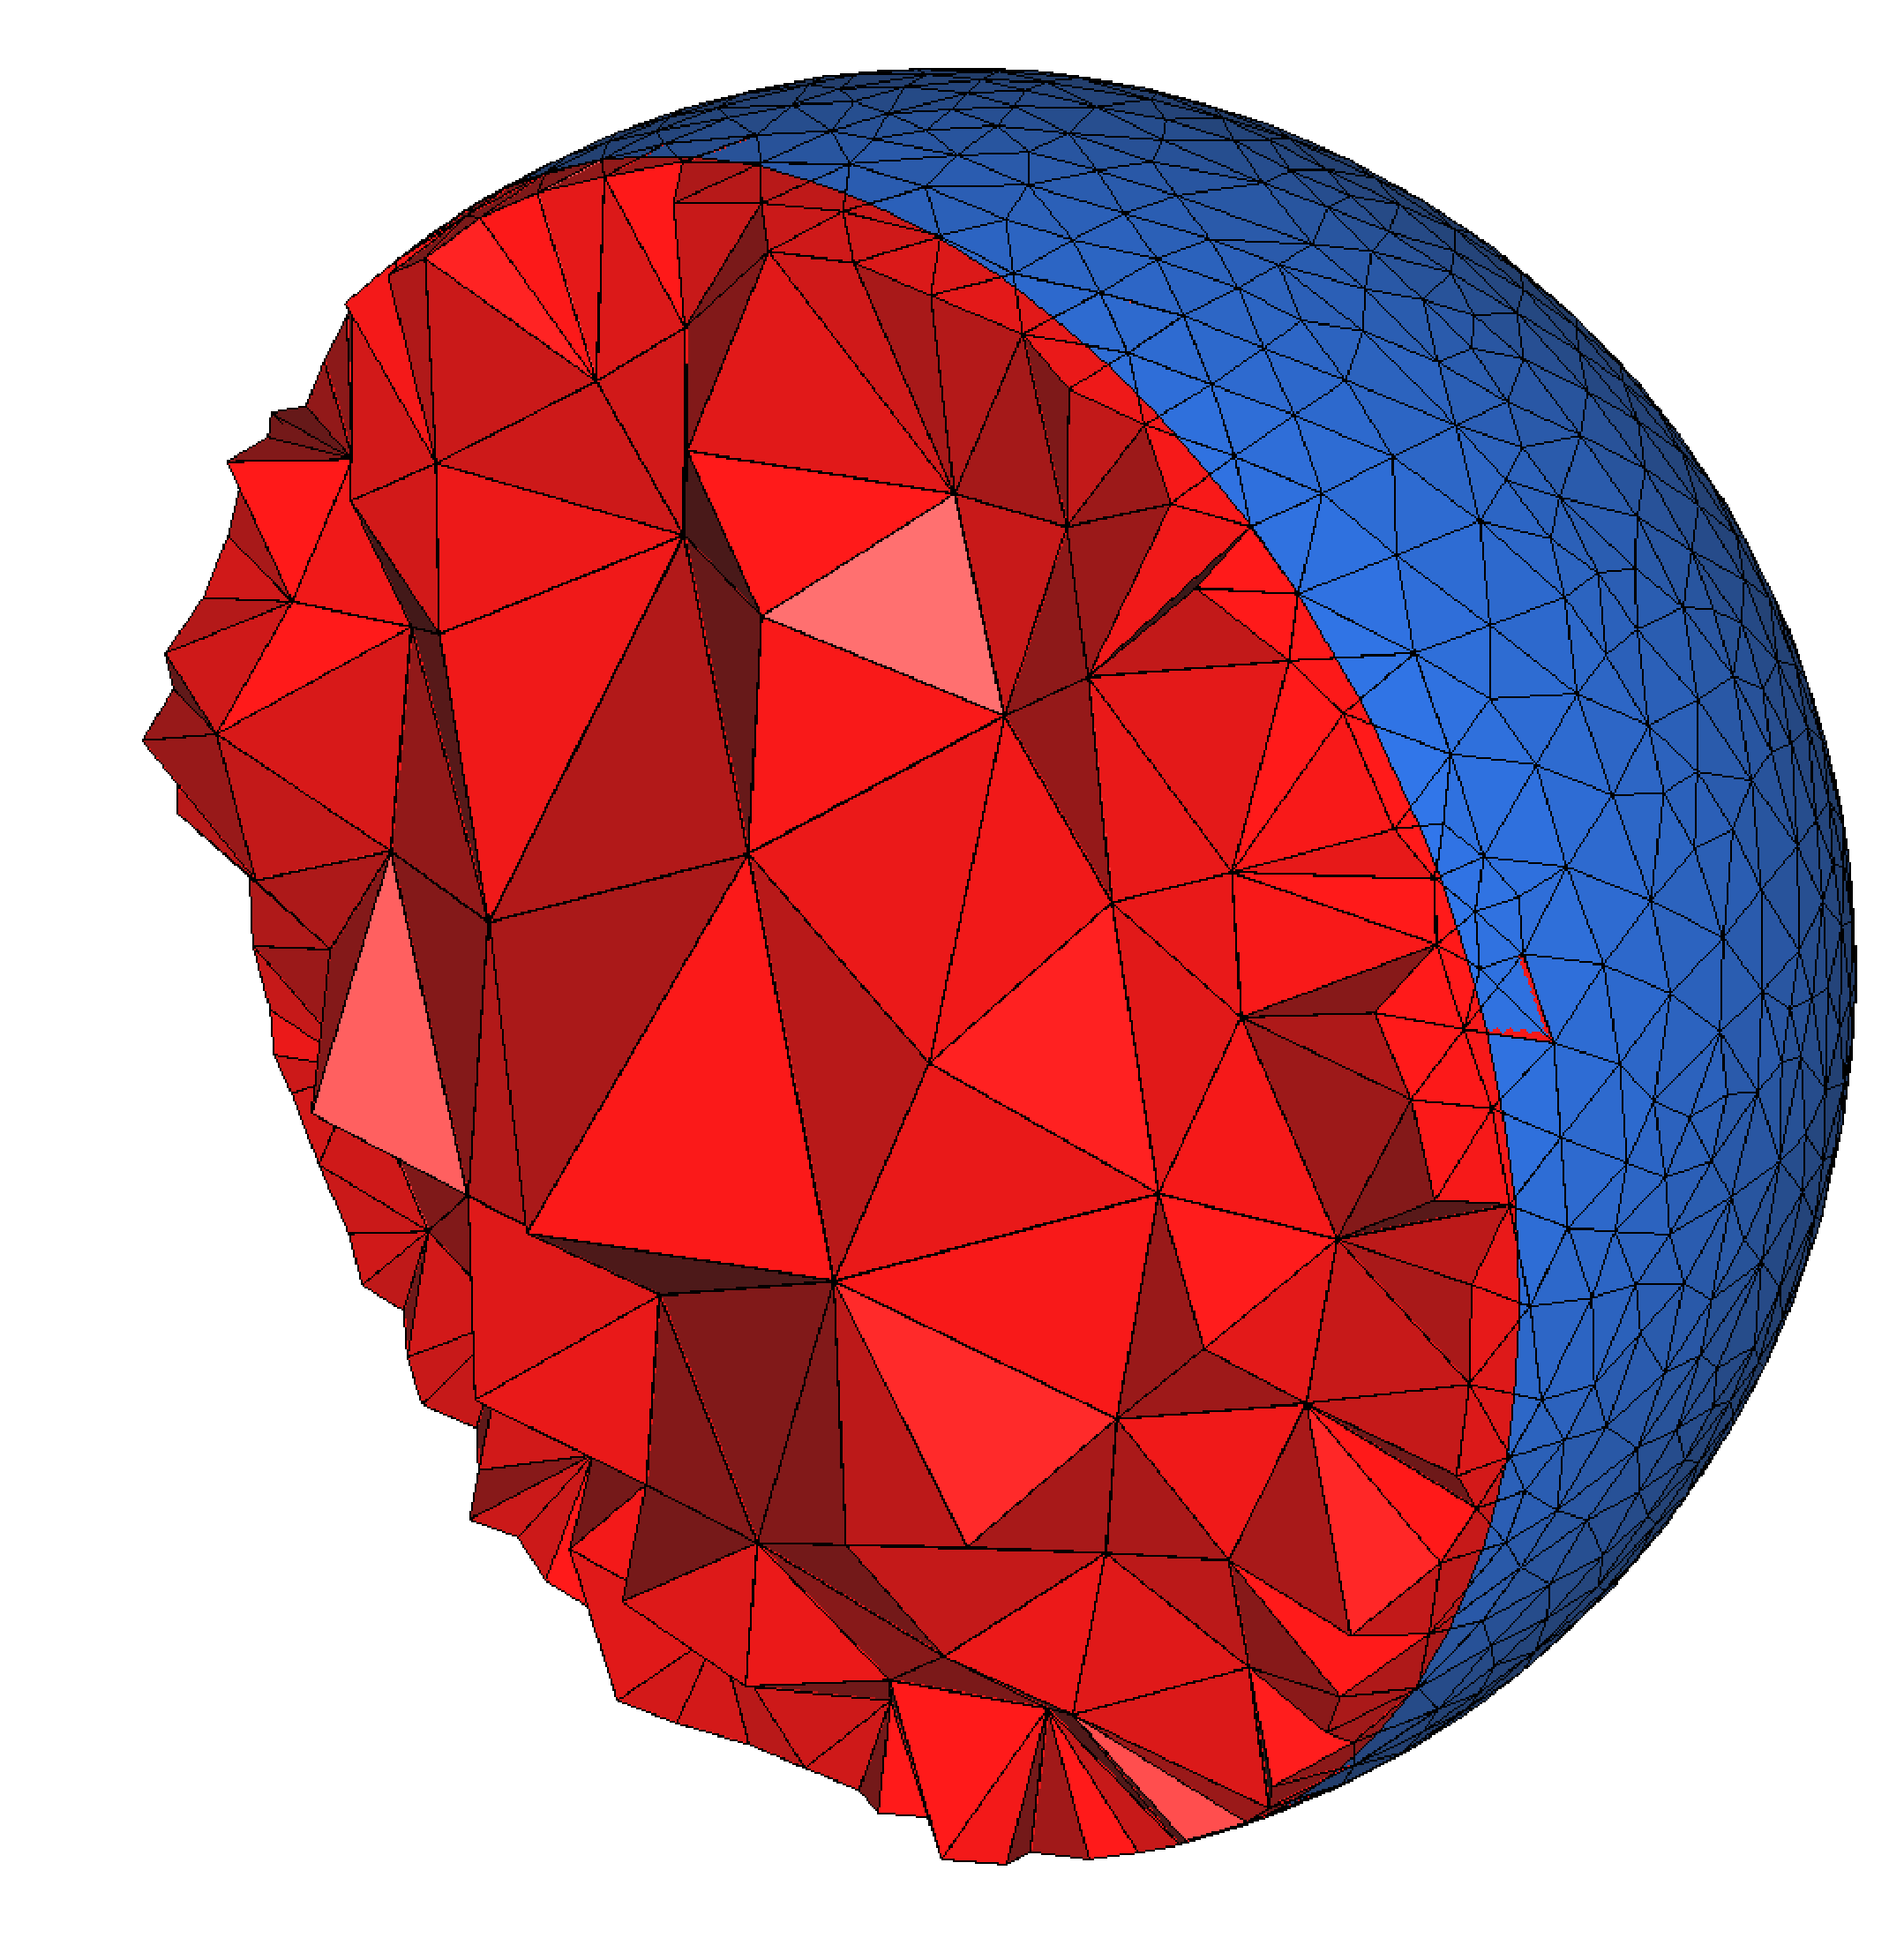
\includegraphics[height=5cm]{Mesh_3/pictures/implicit_domain_4}
   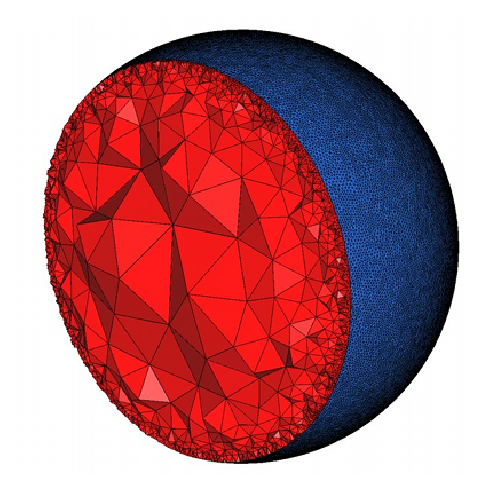
\includegraphics[height=5cm]{Mesh_3/pictures/implicit_domain_5}
 \end{ccTexOnly}
 \begin{ccHtmlOnly}
   <img border="0" height="250px" src="./pictures/implicit_domain.jpg"><br/>
   <img border="0" height="250px" src="./pictures/implicit_domain_3.jpg">
   <img border="0" height="250px" src="./pictures/implicit_domain_4.jpg">
   <img border="0" height="250px" src="./pictures/implicit_domain_5.jpg"><br/>
 \end{ccHtmlOnly}
 \caption{Top : the mesh  is obtained using the parameters $(25,0.15,0.05)$ for the angular bound,
radius bound and distance bound of  surface facets
and 
$(4,0.2)$ for  the radius-edge bound and radius  bound of mesh cells. The result is a  uniform mesh which contains tetrahedra
of about the same size. 
Bottom  left :
the mesh  is obtained by relaxing the \emph{ size bound} of tetrahedra
and facets.
 The result is a small coarse mesh. 
Bottom middle : the mesh  is obtained from the previous one  by tightening the \emph{distance bound} 
of surface facets to
$0.01$. The result is then a graded 3D mesh with a dense surface mesh
achieving a precise approximation. 
Bottom right :
the mesh  is obtained from the previous one  by fixing \emph{radius bound} of surface facets to $0.01$. The surface mesh is then denser to achieve the size bound.}
  \label{figure:parameters}
\end{center}
\end{figure}

\subsubsection{Optimization phase}

The optimization phase is a succession of optimization processes,
including possibly a Lloyd smoothing, an odt-smoothing,
a perturber and an exuder.

The  Lloyd and odt-smoother are global optimizers
 moving the  mesh vertices to  minimize  
a   mesh energy.   Those optimizers are described respectively in 
\cite{cgal:dfg-cvtaa-99t, cgal:dw-tmgob-02} and  in \cite{cgal::c-mssbo-04,cgal:acyd-vtm-05}.
In both case the mesh energy
is  the \ccc{L1}  error  resulting from the interpolation 
of the function $f(x) =x^2$ by a piecewise linear function. 
In the case of Lloyd smoother,
the interpolation  is  linear in each Voronoi cell of the set of  mesh vertices.
In the case of the odt-smoother,  the interpolation is linear in each cell 
of the Delaunay triangulation of the  mesh vertices,
hence the name odt which is an  abbreviation for ``optimal Delaunay triangulation''.
The Lloyd optimizer is known to be blind to the occurrence of slivers in the mesh 
while the odt-smoother tend to chase them out. Both of them are global optimizers, 
meaning that they try to improve
the whole mesh rather than focusing on the worst elements. However, both  are empirically known
to be very efficient as a preliminary step of optimization, as they tend to enhance the
efficiency of the pertuber and/or exuder applied next.

The pertuber and  the exuder focus on improving the worst mesh elements.
The perturber~\cite{cgal:tsa-ps3dd-09} improves the meshes by local changes
in  the vertices positions
aiming to make sliver disappear. The exuder~\cite{cgal:cdeft-slive-00}
chases the remaining slivers by turning the Delaunay mesh into a 
weighted Delaunay mesh with optimal weights affected to the vertices.

 Each optimization process
can be activated or not,
 according to the user requirements
and the available time. 
By default, only the perturber and  the exuder are activated.
For a maximum efficiency, whatever  may be the optimization processes activated,
they should be launched in the order that is a suborder 
of the following:
\ccc{odt-smoother}, \ccc{Lloyd-smoother}, \ccc{perturber},
\ccc{exuder}. No smoother or perturber can be launched after an exudation process.



\section{Interface}
\label{Mesh_3_section_interface}

A 3D mesh generation  process is launched through a call
 to   one of the two following functions:
 
\ccGlobalFunction{
  template <class C3T3,
  class MeshDomain,
  class MeshCriteria>
  C3T3 make_mesh_3(MeshDomain domain, 
                   MeshCriteria criteria,
                   parameters::internal::Lloyd lloyd = parameters::no_lloyd(),
                   parameters::internal::Odt odt = parameters::no_odt(),
                   parameters::internal::Perturb perturb = parameters::perturb(),
                   parameters::internal::Exude exude = parameters::exude()); }{}
             

\ccGlobalFunction{
  template <class C3T3,
  class MeshDomain,
  class MeshCriteria>
  void refine_mesh_3(C3T3& c3t3,
                     MeshDomain domain,
                     MeshCriteria criteria,
                    parameters::internal::Lloyd lloyd = parameters::no_lloyd(),
                    parameters::internal::Odt odt = parameters::no_odt(),
                    parameters::internal::Perturb perturb = parameters::perturb(),
                    parameters::internal::Exude exude = parameters::exude()); }{}


The function \ccc{make_mesh_3} generates from scratch a mesh
of the input domain, while
the function \ccc{refine_mesh_3} refines
an existing mesh of the input domain.

The template parameter \ccc{C3T3} is required to be a model of
the concept 
\ccc{MeshComplex_3InTriangulation_3}, a data structure devised to
represent a three dimensional complex embedded in a 3D
triangulation. In both functions,  an instance  of type \ccc{C3T3} is used to maintain the current
approximating simplicial mesh of the domain and subdomains
and to represent the final  3D mesh at the end
of the procedure.
The type \ccc{C3T3} is   required to provide a nested type
\ccc{C3T3::Triangulation_3} for the 3D triangulation
embedding the mesh. This triangulation is required to be a regular
triangulation.
 The vertex and cell base classes of the
triangulation \ccc{C3T3::Triangulation_3} are required to be respectively  models of the
concepts \ccc{MeshVertexBase_3} and \ccc{MeshCellBase_3}.

The template parameter \ccc{MeshDomain} is required to be a model of
the concept  \ccc{MeshDomain_3}. The argument \ccc{domain} of type
\ccc{MeshDomain}
 is the sole link through which the domain
to be discretized is known  by the mesh generation algorithm. 
The concept \ccc{MeshDomain_3} is similar to the concept \ccc{SurfaceMeshTraits} 
defined by the surface mesh generation package.
This concept  provides, among others,
  member functions to test whether or not
a query segment intersects boundary surfaces,
and to compute an intersection point  in the affirmative.
The \ccc{MeshDomain_3} concept adds  member functions 
which given a query point tell whether the point lies
inside or outside the domain and in which subdomain the point lies
if inside.

% There are compatibility requirements between the template parameter 
% \ccc{C3T3} and \ccc{MeshDomain}.
% The nested types \ccc{MeshDomain::Subdomain_index},
% and \ccc{MeshDomain::Index} 
% have to be convertible respectively
% to the nested types \ccc{C3T3::Triangulation::Cell::Subdomain_index}
% and  \ccc{C3T3::Triangulation::Vertex::Index}.

The template parameter \ccc{MeshCriteria} must be a model of the concepts
\ccc{MeshCriteria_3}. 
The argument of
type \ccc{MeshCriteria} passed to the mesh generator specifies the
size and shape requirements for the tetrahedra in the mesh
and for the triangles in the boundary surface mesh. These criteria
condition the rules that drive the refinement process.  At the end 
of the refinement process, mesh elements satisfy the criteria.
This may not be strictly true anymore after the optimization phase, but this
last phase is devised to only improve the mesh quality.


The   four  additional parameters  are optimization parameters.
They control which optimization processes are performed
and allow the user  to tune the parameters of the activated  optimization processes.
These parameters have internal types which are not described
but the library provides two global functions for each, to generate
appropriate values:
\begin{itemize}
\item \ccc{parameters::lloyd()} and \ccc{parameters::no_lloyd()} activate or deactivate  the Lloyd smoother.
 \item \ccc{parameters::odt()} and \ccc{parameters::no_odt()} activate or deactivate the odt-smoother.
\item \ccc{parameters::perturb()} and \ccc{parameters::no_perturb()} activate or deactivate the perturber.
\item \ccc{parameters::exude()} and \ccc{parameters::no_exude()} activate or deactivate the exuder.
\end{itemize}


These parameters are optional and can be passed in any order.
If one parameter is not passed the default value is used. By default,
only the perturber and the exuder are activated.
Note that whatever may be the optimization processes activated by \ccc{make_mesh_3}
or \ccc{refine_mesh_3},
they are always launched in the order that is a suborder 
of the following:
\ccc{odt smoother}, \ccc{Lloyd smoother}, \ccc{perturber} and 
\ccc{exuder}.


The package also provides four global functions to launch
each optimization process independently. These functions are useful for advanced experimentation 
on the efficiency of each optimization method.
Note however that the exuder adds on mesh vertices  weights that are conditioned by vertices
positions. Therefore an exudation process should never be run before
a smoother or a perturber. 

\ccSetThreeColumns{Mesh_optimization_return_code}{lloyd_optimize_mesh_3(C3T3& c3t3, MeshDomain domain)}{}
\ccGlobalFunction{
	template< C3T3,  MeshDomain>
	Mesh_optimization_return_code lloyd_optimize_mesh_3(C3T3& c3t3, MeshDomain domain);}{}
%, double time_limit=0, double sliver_bound=0,
%	int max_iteration_nb=0, double? convergence=0)
%\ccGlue
\ccGlobalFunction{
	template< C3T3,  MeshDomain>
	Mesh_optimization_return_code odt_optimize_mesh_3(C3T3& c3t3, MeshDomain domain);}{}
%, double time_limit=0, double sliver_bound=0,
%	int max_iteration_nb=0, double? convergence=0
%\ccGlue
\ccGlobalFunction{
	template< C3T3,  MeshDomain>
	Mesh_optimization_return_code perturb_mesh_3(C3T3& c3t3, MeshDomain domain);}{}
%, double time_limit=0, double sliver_bound=0
%\ccGlue
\ccGlobalFunction{
	template< C3T3>
	Mesh_optimization_return_code exude_mesh_3(C3T3& c3t3);}{}
%, double time_limit=0, double sliver_bound=0



\section{Examples}
\label{Mesh_3_section_examples}


\subsection{Mesh Generation From an Implicit Domain}
The following code produces a 3D mesh for a domain whose boundary surface
is defined by an implicit
function. Figure~\ref{figure:implicit_domain} shows a cut view of the
resulting mesh.

\ccIncludeExampleCode{Mesh_3/mesh_implicit_sphere.cpp}

\begin{figure}[ht]
\begin{center}
 \begin{ccTexOnly}
   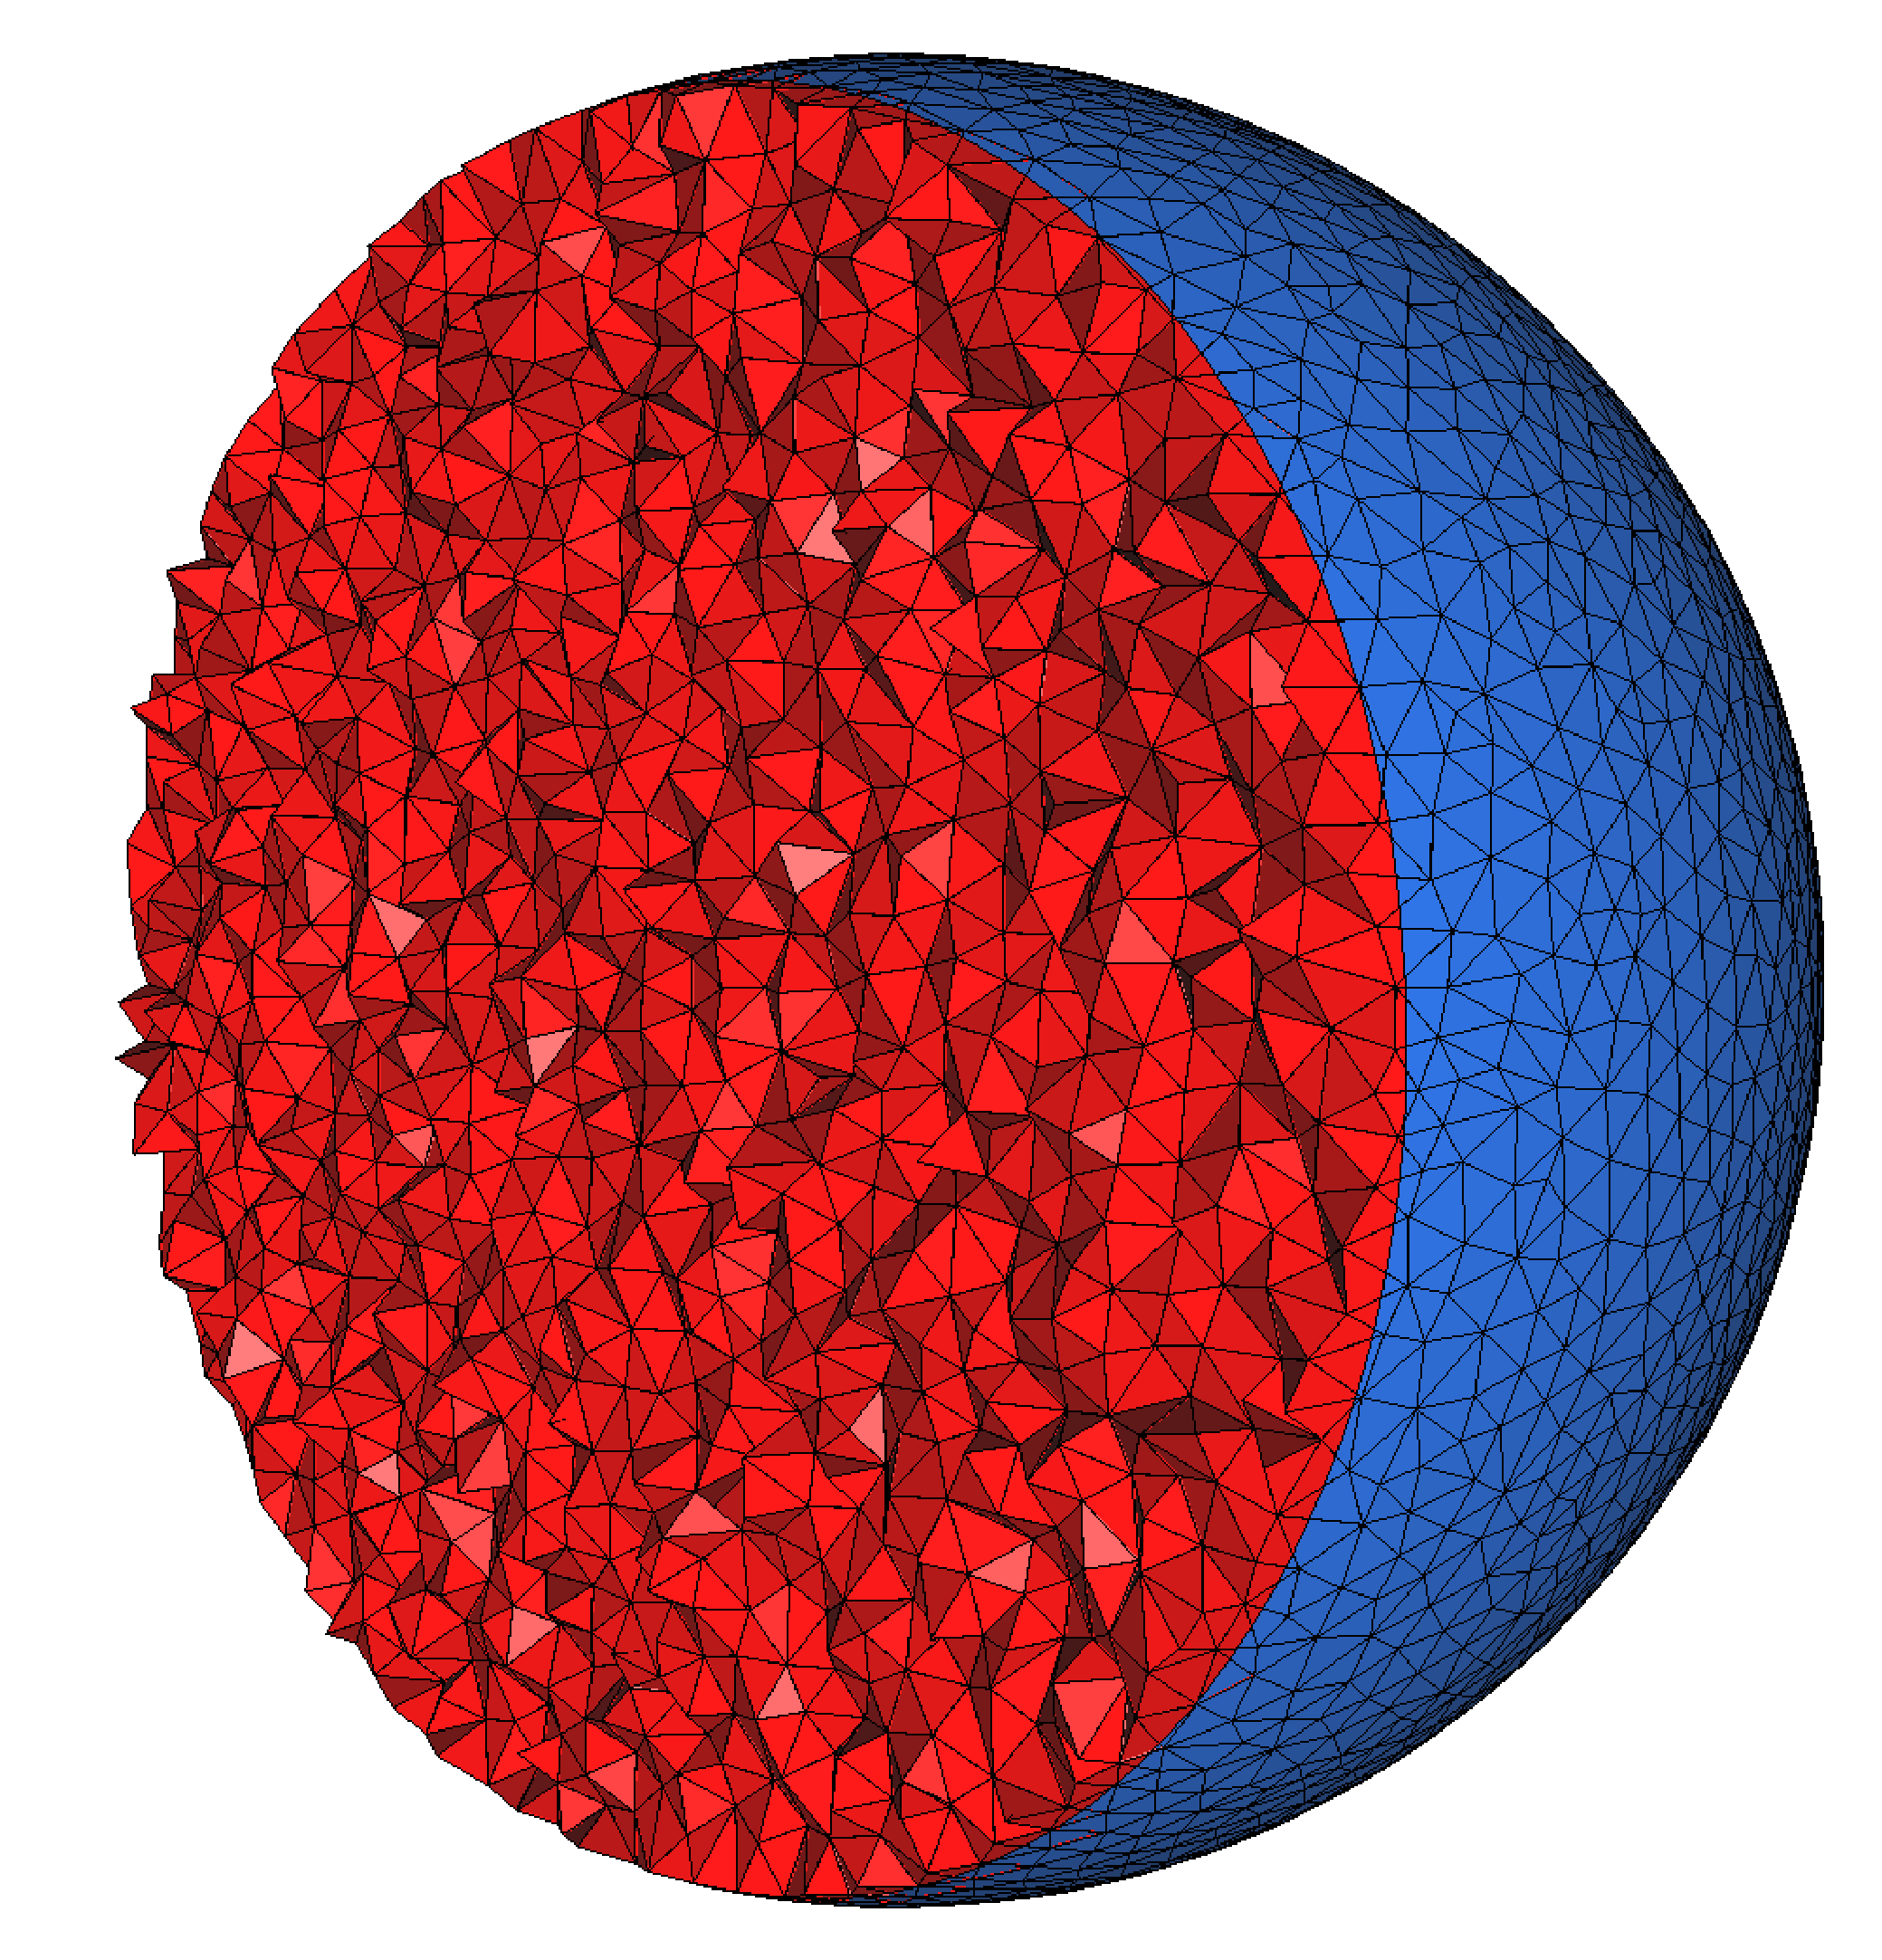
\includegraphics[height=6cm]{Mesh_3/pictures/implicit_domain}
 \end{ccTexOnly}
 \begin{ccHtmlOnly}
   <img border="0" src="./pictures/implicit_domain.jpg"><br/>
 \end{ccHtmlOnly}
 \caption{Cut-View of a 3D mesh produced from an implicit domain}
  \label{figure:implicit_domain}
\end{center}
\end{figure}


\subsection{Mesh Generation From a Polyhedral Domain}
\label{Mesh_3_subsection_examples_polyhedral}
The following code produces a 3D mesh for a domain
defined by polyhedral surfaces. Figure~\ref{figure:polyhedral_domain}
shows the resulting mesh.

\ccIncludeExampleCode{Mesh_3/mesh_polyhedral_domain.cpp}

\begin{figure}[ht]
\begin{center}
 \begin{ccTexOnly}
   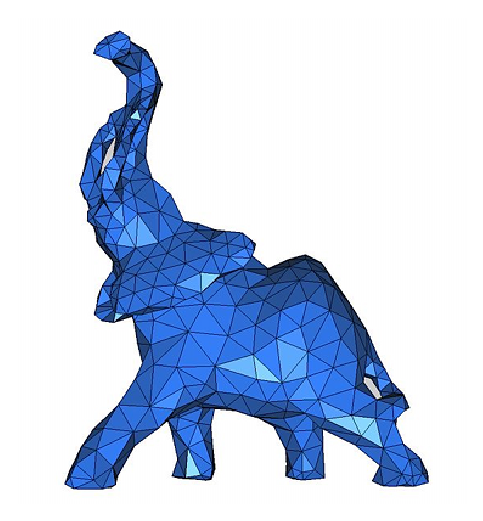
\includegraphics[height=7cm]{Mesh_3/pictures/polyhedral_domain}
   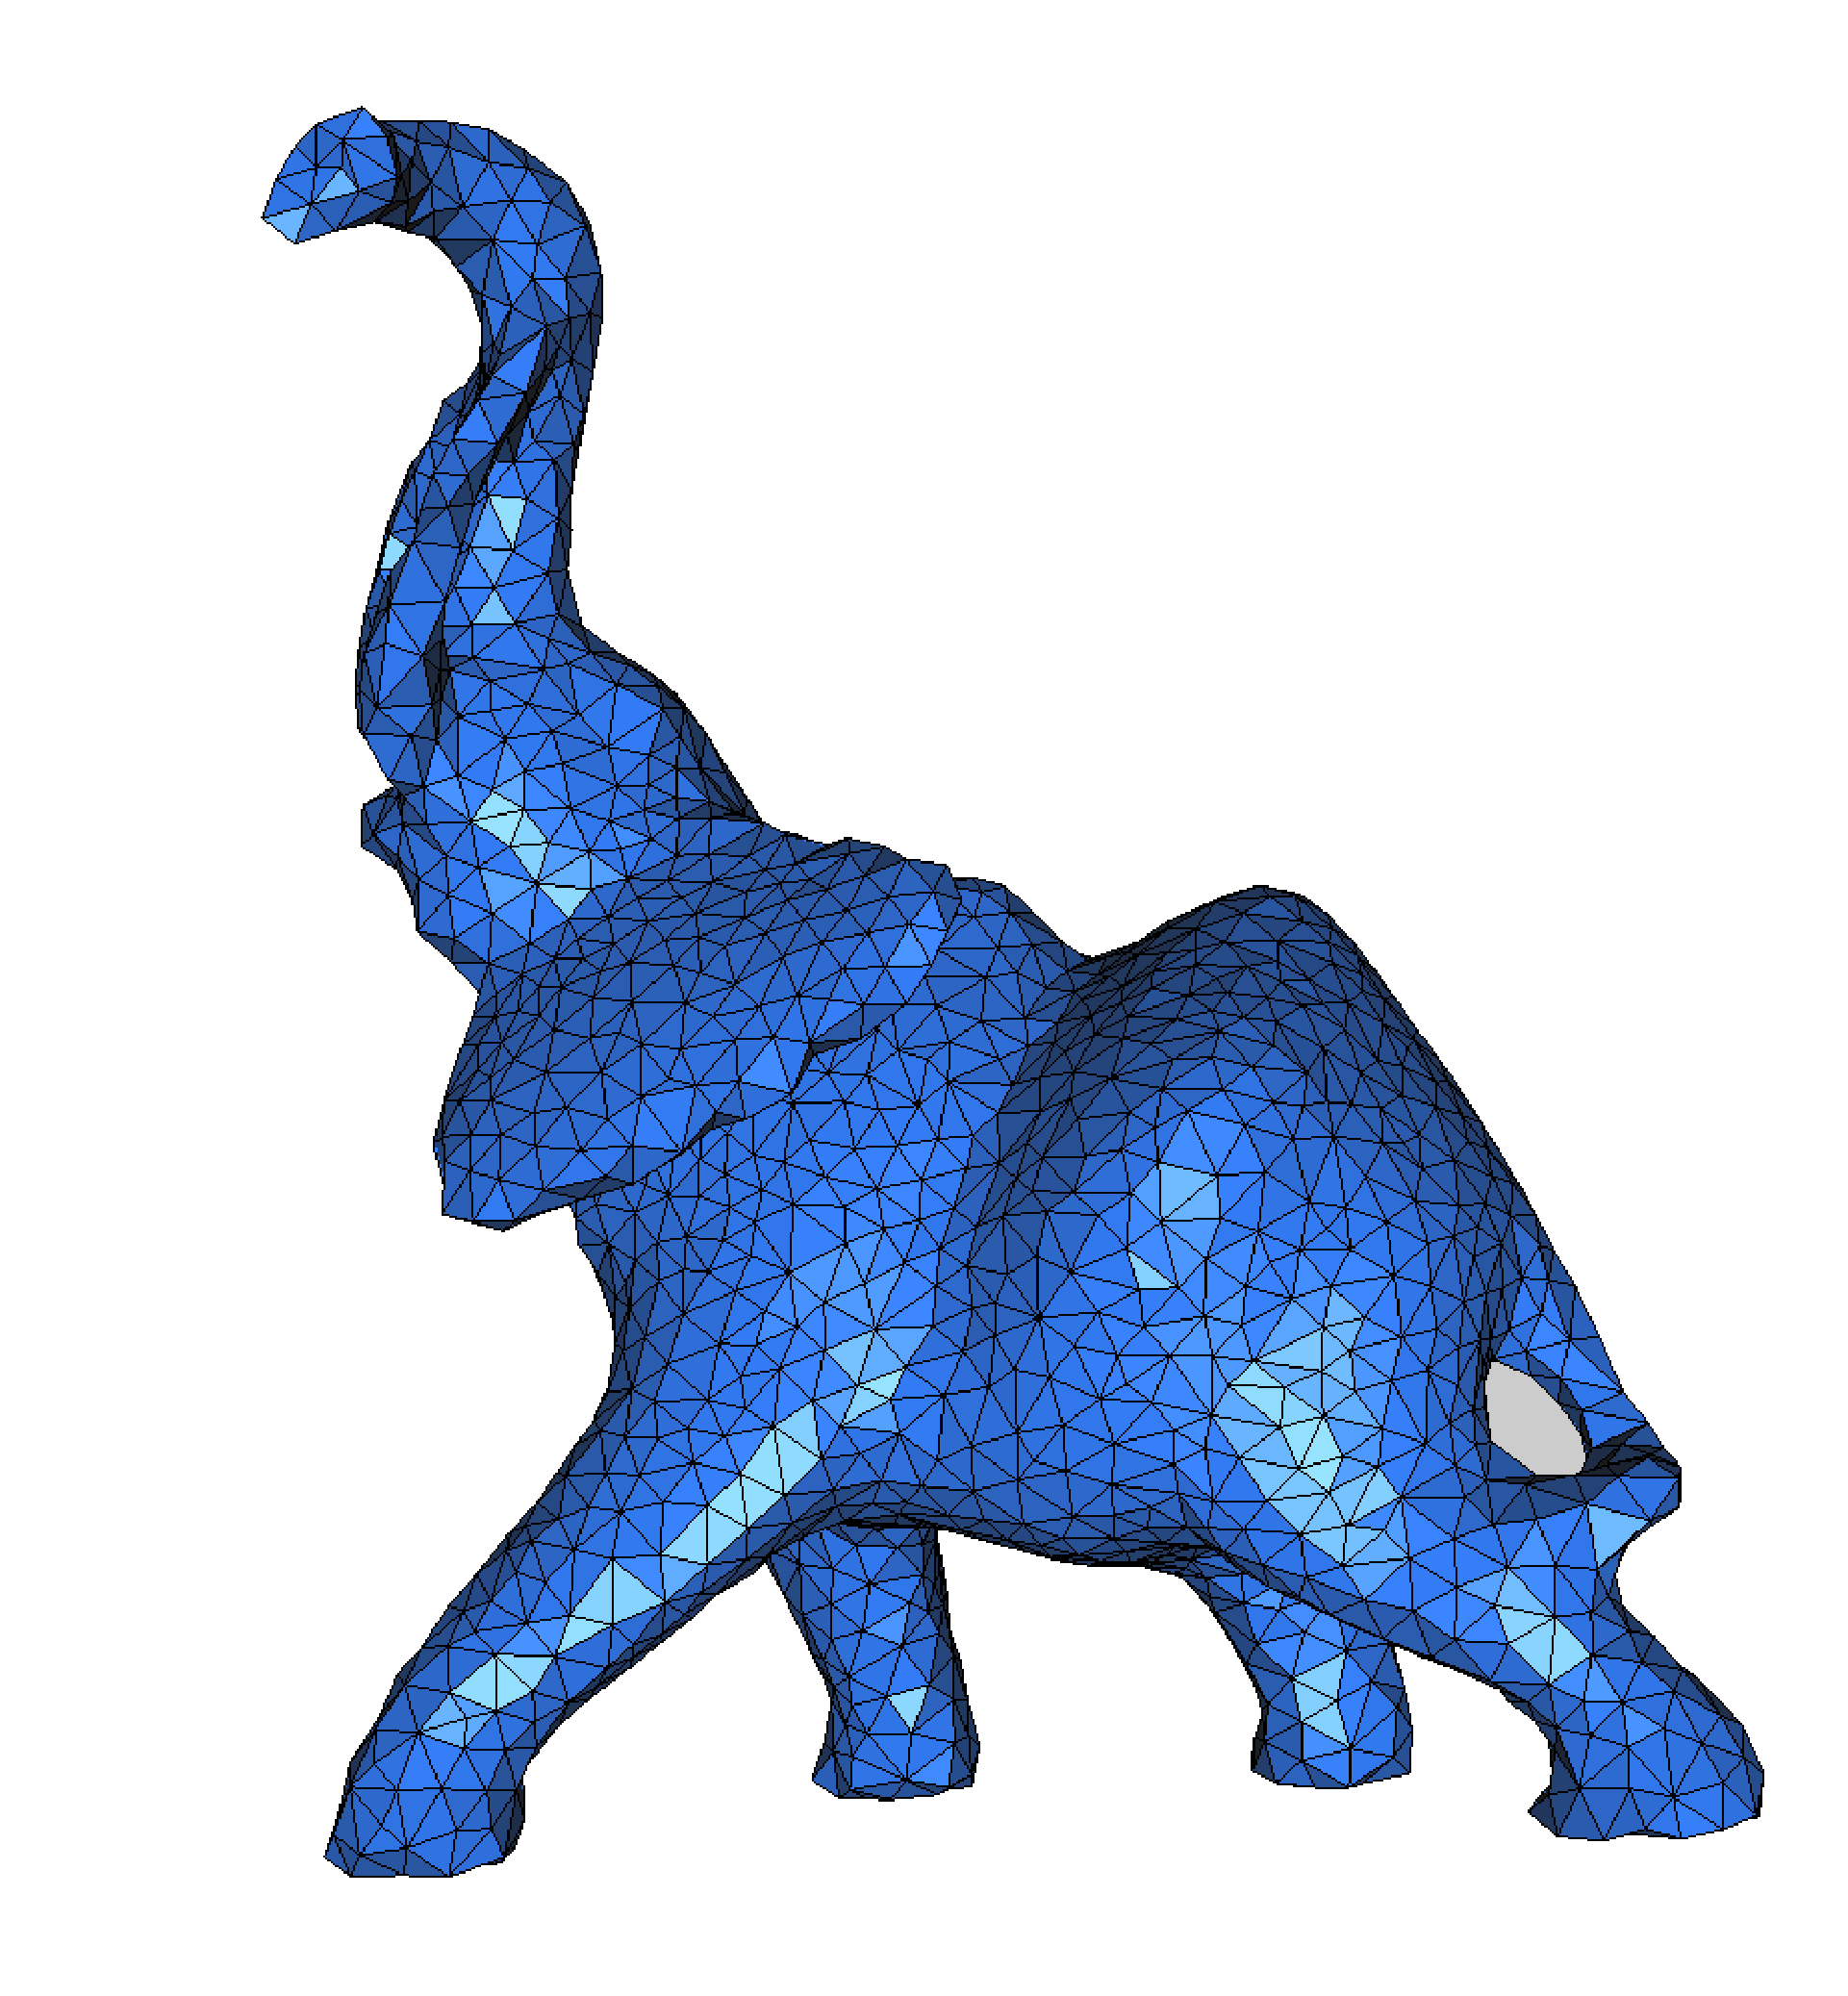
\includegraphics[height=7cm]{Mesh_3/pictures/polyhedral_domain_2}
 \end{ccTexOnly}
 \begin{ccHtmlOnly}
   <img border="0" src="./pictures/polyhedral_domain.jpg">
   <img border="0" src="./pictures/polyhedral_domain_2.jpg"><br/>
 \end{ccHtmlOnly}
 \caption{View of 3D meshes produced from a polyhedral domain. (i) 
   is a view of file out\_1.mesh and (ii) is a view of file
   out\_2.mesh. Code from
   subsection~\ref{Mesh_3_subsection_examples_polyhedral} generates
   these files.}
  \label{figure:polyhedral_domain}
\end{center}
\end{figure}


\subsection{Mesh Generation From a Segmented 3D Image}
\label{Mesh_3_subsection_examples_3d_image}
The following code produces  a 3D mesh from
a 3D image. The image is a segmented medical image  in which each 
voxel  is associated a label  in accordance with
the tissue  the voxel belongs to.
The domain is therefore a multi-domain
where each subdomain corresponds to a specific tissue.
The resulting mesh is shown in Figure~\ref{figure:liver_3d_image_mesh}.

\ccIncludeExampleCode{Mesh_3/mesh_3D_image.cpp}

\begin{figure}[ht]
\begin{center}
 \begin{ccTexOnly}
   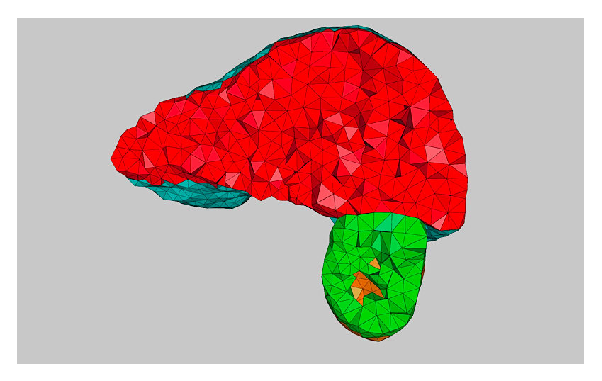
\includegraphics[width=10cm]{Mesh_3/pictures/liver}
 \end{ccTexOnly}
 \begin{ccHtmlOnly}
   <img border="0" src="./pictures/liver.jpg"><br/>
 \end{ccHtmlOnly}
 \caption{Cut-view of a 3D mesh produced from a segmented liver image. Code from
 subsection~\ref{Mesh_3_subsection_examples_3d_image} generates this file.}
  \label{figure:liver_3d_image_mesh}
\end{center}
\end{figure}

% \subsection{Mesh Generation with explicit optimization step}

% The following code produces a 3D mesh for a monodomain whose boundary surface
% is defined by an implicit ellipsoid
% function. This example shows how default optimization step of \ccc{make_mesh_3} could
% be disabled, and how optimization functions may be called instead.

% Figure~\ref{figure:dihedral_angle_distribution} shows the dihedral angle distribution of
% the meshes generated by the following code.

% \begin{figure}[ht]
% \begin{center}
%  \begin{ccTexOnly}
%    \includegraphics[width=14cm]{Mesh_3/pictures/dihedral_angle_distribution}
%  \end{ccTexOnly}
%  \begin{ccHtmlOnly}
%    <img border="0" src="./pictures/dihedral_angle_distribution.png"><br/>
%  \end{ccHtmlOnly}
%  \caption{Dihedral angle distribution before and after optimization step.}
%   \label{figure:dihedral_angle_distribution}
% \end{center}
% \end{figure}

% \ccIncludeExampleCode{Mesh_3/mesh_implicit_ellipsoid.cpp}


\subsection{Tuning mesh optimization}
\label{Mesh_3_subsection_examples_optimization}

In the previous examples, the mesh generation is launched through a  call
\ccc{make_mesh_3(domain,criteria)} with a minimal number of parameters. In such cases, 
the default optimization strategy is applied: after the Delaunay refinement process
 two optimization steps are performed, a perturbation and  a sliver exudation.
The following examples show how to disable default optimization steps 
and how to tune the parameters of optimization steps.



\subsubsection{Disabling exudation and tuning perturbation}

In this first example, we show how to disable the exudation step.
The optimization phase after the refinement includes only
a perturbation phase which is launched  with no time bound
and an objective of 10 degrees for the minimum dihedral angle
of the mesh.
The example shows two ways of achieving the same result. The first way
issues a single call to \ccc{make_mesh_3} with the required optimization 
process activated and tuned. In the second way, \ccc{make_mesh_3} is first called
without any optimization process and the resulting mesh is next optimized
through a call to \ccc{perturb_mesh_3} with tuned parameters.

\ccIncludeExampleCode{Mesh_3/mesh_optimization_example.cpp}


\subsubsection{Using Lloyd global optimization}

In this second example, we show how to call  the Lloyd optimization on the
mesh, followed by a call to exudation. We set a time bound of 30s for the Lloyd optimization. 
We set a  time bound of 10s for the exuder and a sliver bound of 10 degrees.

\ccIncludeExampleCode{Mesh_3/mesh_optimization_lloyd_example.cpp}





\section{Performances}

We provide some performance numbers about our mesh generation engine. The machine
used is a PC running Linux64 with two Intel Xeon CPU X5450 clocked at 3.00 GHz
with 32GB of RAM. The program has been compiled with g++ v4.3.2 with the -O3 option. 
Note that our implementation does not take advantage of multi-core
architectures.

\subsection{Delaunay refinement}

We study the refinement part of the mesh generation engine in this section. We
give CPU time (measured by \ccc{CGAL::Timer}) using the 3 provided oracles. In all experiments, we produce well
shaped elements: we set facet angle bound and radius edge bound to their
theoretical limit (resp. 30 degrees and 2). We also use the same size for facets
and cells.

\subsubsection{Implicit function}

We mesh an analytical sphere of radius 1.

\begin{center}
\begin{tabular}{|l|l|l|l||c|}
  \hline
  Size bound & vertices nb & facets nb & tetrahedra nb & CPU Time (s) \\
  \hline
  0.4 & 358 & 394 & 1,546 & 0.047 \\
  0.2 & 2,306 & 1,524 & 12,100 & 0.295 \\
  0.1 & 16,832 & 6,234 & 97,109 & 2.46 \\
  0.05 & 127,865 & 24,868 & 776,098 & 22.9 \\
  0.025 & 996,256 & 100,404 & 6,204,502 & 204 \\
  \hline
\end{tabular}
\end{center}

\subsubsection{Polyhedral domain}

\begin{figure}[ht]
\begin{center}
 \begin{ccTexOnly}
   \includegraphics[width=10cm]{Mesh_3/pictures/bench_polyhedral.jpg}
 \end{ccTexOnly}
 \begin{ccHtmlOnly}
   <img border="0" src="./pictures/bench_polyhedral.jpg"><br/>
 \end{ccHtmlOnly}
 \caption{View of polyhedral mesh generation result (size = 0.005).}
  \label{figure:mesh_3_benchmark_polyhedral}
\end{center}
\end{figure}

We mesh a volume bounded by a close triangulated surface made of about 50,000 vertices and 100,000 triangles.
Picture~\ref{figure:mesh_3_benchmark_polyhedral} shows the mesh obtained when
size is set to 0.005.

\begin{center}
\begin{tabular}{|l|l|l|l||c|}
  \hline
  Size bound & vertices nb & facets nb & tetrahedra nb & CPU Time (s) \\
  \hline
  0.04 & 397 & 674 & 1,262 & 0.339 \\
  0.02 & 2,697 & 3,547 & 11,177 & 2.70 \\
  0.01 & 18,176 & 15,578 & 90,480 & 19.7 \\
  0.005 & 129,377 & 64,793 & 721,355 & 152 \\
  \hline
\end{tabular}
\end{center}

\subsubsection{3D image}

\begin{figure}[ht]
\begin{center}
 \begin{ccTexOnly}
   \includegraphics[width=14cm]{Mesh_3/pictures/bench_3d.jpg}
 \end{ccTexOnly}
 \begin{ccHtmlOnly}
   <img border="0" src="./pictures/bench_3d.jpg"><br/>
 \end{ccHtmlOnly}
 \caption{View of 3d image mesh generation result (size = 4).}
  \label{figure:mesh_3_benchmark_3d_image}
\end{center}
\end{figure}

We mesh image number 2 from the 3D-IRCADb-01\footnote{available at \lcTex{\url{http://www.ircad.fr/softwares/3Dircadb/3Dircadb1/index.php}} \lcRawHtml{<A href="http://www.ircad.fr/softwares/3Dircadb/3Dircadb1/index.php">http://www.ircad.fr/softwares/3Dircadb/3Dircadb1/index.php</A>}} public database.
The size of this image is 512x512x172 voxels (about 45M voxels). The size of the voxels
is 0.78mm x 0.78mm x 1.6mm. Picture~\ref{figure:mesh_3_benchmark_3d_image}
shows the mesh obtained for size set to 4.

\begin{center}
\begin{tabular}{|l|l|l|l||c|}
  \hline
  Size bound (mm) & vertices nb & facets nb & tetrahedra nb & CPU Time (s) \\
  \hline
  16 & 3,743 & 3,735 & 19,886 & 0.880 \\
  8 & 27,459 & 19,109 & 159,120 & 6.97 \\
  4 & 199,328 & 76,341 & 1,209,720 & 54.1 \\
  2 & 1,533,660 & 311,420 & 9,542,295 & 431 \\
  \hline
\end{tabular}
\end{center}

%\subsection{Mesh optimization}

%\subsubsection{Exudation}

\section{Design and Implementation History}

Work on the package \ccc{Mesh_3} started during the PhD thesis of Laurent Rineau
advised by Mariette Yvinec.  A first version of the specifications
and code came out of their collaboration.

From the beginning of 2009, most of the work has been performed by St\'ephane
Tayeb, in collaboration with Mariette Yvinec, Laurent Rineau, Pierre Alliez and Jane Tournois.
First, St\'ephane released the first public version of the package, implementing the specifications
written by Laurent and Mariette. 

Since then, St\'ephane added the optimization processes which are
heavily based on the work of Jane Tournois and Pierre Alliez
during the PhD of Jane advised by Pierre.

In collaboration with Laurent Rineau, St\'ephane also added demos and examples.

